\section{Результаты вычислений}
Для решения задачи был выбран язык программирования Python 3.8. Предобработку данных было решено реализовывать при помощи Python 3.8.
В качестве библиотеки для реализации нейронной сети была выбрана библиотека Keras, включенная в библиотеку Tensorflow 2.4.1.

Для создания датасета был разработан веб-сервис на NodeJS, Javascript, HTML, CSS, который позволяет записывать команды и сохранять их в нужном для программы предобработки формате. Также это позволило записать необходимое количество дикторов, которые смогли довольно быстро наговорить команды.


Было проведено 3 вычислительных эксперимента для нейронной сети типа CNN. Структура сети приведена на рисунке \ref{fig:cnn_model}.

\begin{figure}[H]
  \[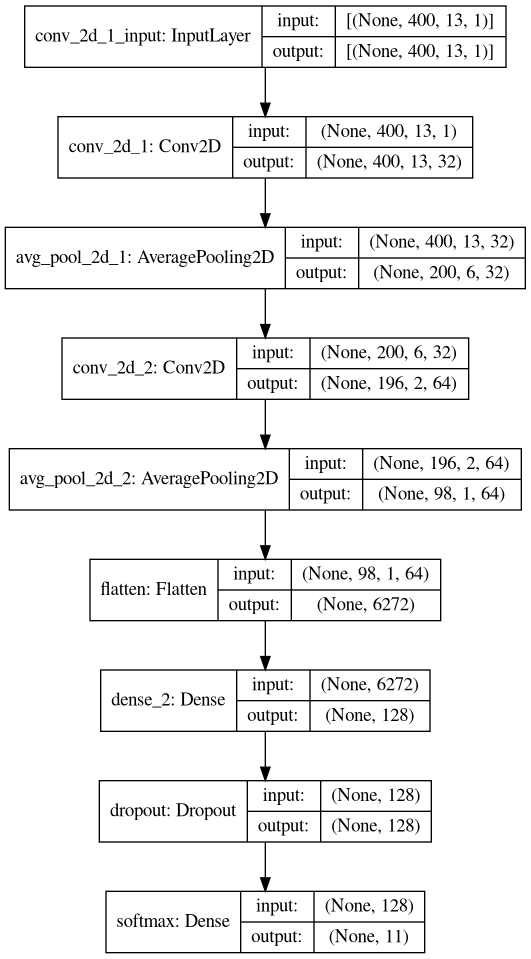
\includegraphics[scale=0.4]{cnn_model.png}\]
  \caption{Структура модели нейронной сети типа CNN}
  \label{fig:cnn_model}
\end{figure}

Все звуковые файлы были предобработаны при помощи алгоритма MFCC.
Звуковая дорожка делится на фреймы. Каждый фрейм - отрезок звуковой дорожки длительностью 20 мс. Каждый фрейм начинается с момента (10 мс. $\times$ номер\_фрейма), нумерация начинается с 0. Для каждой звуковой дорожки количество фреймов - 400. Если количество фреймов у дорожки меньше 400, то слева и справа добавляются нули. Это число было выбрано как максимально возможное количество фреймов для всех дорожек. Количество коэффициентов в алгоритме MFCC - 13, количество фильтров - 26. В итоге размерность данных, поступающих на вход нейронной сети - $400\times13$.

Датасет состоит из 6 дикторов. Каждый диктор записал 11 команд : 'back', 'down', 'menu', 'off', 'on', 'open', 'play', 'power', 'stop', 'up', 'volume'.
\\

\begin{tabular}[c]{ | p{2cm} | p{2cm} | p{6cm} | p{4cm} | }
\hline
Диктор & Тип голоса & Кол-во звук. дорожек на каждую команду & Сумм. кол-во звук. дорожек  \\ \hline
speaker1 & Мужской & 50 & 550 \\
speaker2 & Мужской & 40 & 440 \\
speaker3 & Мужской & 40 & 440 \\
speaker4 & Мужской & 40 & 440 \\
speaker5 & Мужской & 50 & 550 \\
speaker6 & Женский & 50 & 550 \\ \hline
\end{tabular}
\\

Первый эксперимент: нейронная сеть обучается на первом дикторе с мужским голосом, тестирование производится на каждом дикторе. 

Второй эксперимент: нейронная сеть обучается на всех дикторах с мужским голосом, тестирование производится на каждом дикторе. 

Третий эксперимент: нейронная сеть обучается на всех дикторах, тестирование производится на каждом дикторе.

Датасет предварительно разделяется на тренировочную и тестовую части. На тренировочную часть отводится 70\% данных диктора, на тестовую часть - 30\%. В процессе тренировки после каждой эпохи тренировочные данные перемешиваются. 15\% тренировочных данных в каждой эпохе - валидационные. В качестве метрики для оценки эффективности была выбрана метрика точности (accuracy), а для валидации - функция потерь категориальной кросс-энтропии (val\_loss). Алгоритм оптимизации - Adam. Максимальное количество эпох - 50. Если значение метрики val\_loss не уменьшается в течение 20 эпох, то обучение останавливается.

Графики обучения для каждого из экспериментов приведены на рисунках \ref{fig:cnn_speaker1_train_graphs}, \ref{fig:cnn_all_male_speakers_train_graphs}, \ref{fig:cnn_all_speakers_train_graphs}.

В конце каждого эксперимента проводится тестирование нейронной сети.
А в случае обучения на all\_speakers помимо тестирования производится построение матрицы ошибок (confusion matrix) для каждого диктора и для каждого из четырех пороговых значений: 0.5, 0.6, 0.7, 0.8. Матрицы представлены на рисунке \ref{fig:cnn_cm_all_speakers}.

Результаты тестирования представлены в таблице \ref{table:test_summary}. Обозначения, которые используются:

all\_speakers = [speaker1, speaker2, speaker3, speaker4, speaker5, speaker6]

all\_male\_speakers = [speaker1, speaker2, speaker3, speaker4, speaker5]

\begin{figure}[H]
  \[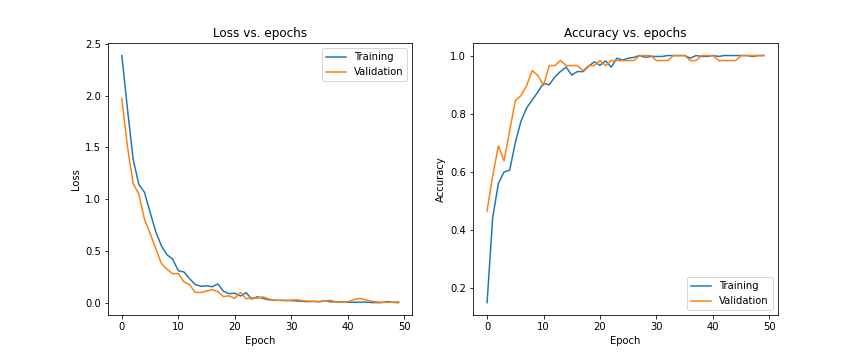
\includegraphics[scale=0.4]{cnn_speaker1_train_graphs.png}\]
  \caption{Графики функции потерь и точности в течение обучения на speaker1}
  \label{fig:cnn_speaker1_train_graphs}
\end{figure}

\begin{figure}[H]
  \[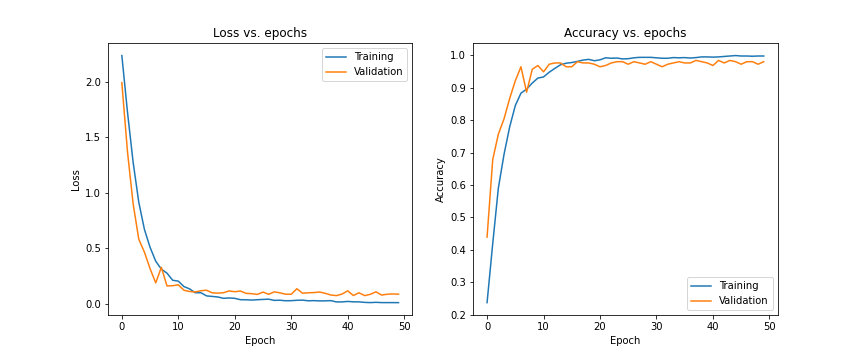
\includegraphics[scale=0.4]{cnn_all_male_speakers_train_graphs.png}\]
  \caption{Графики функции потерь и точности в течение обучения на all\_male\_speakers}
  \label{fig:cnn_all_male_speakers_train_graphs}
\end{figure}

\begin{figure}[H]
  \[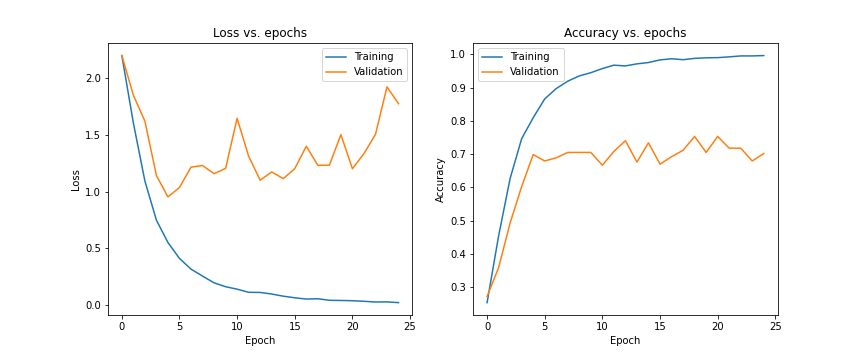
\includegraphics[scale=0.4]{cnn_all_speakers_train_graphs.png}\]
  \caption{Графики функции потерь и точности в течение обучения на all\_speakers}
  \label{fig:cnn_all_speakers_train_graphs}
\end{figure}


\begin{table}
\small
\centering
\csvautotabular[respect underscore=true]{csv/test_summary.csv}
\caption{Результаты вычислений}
\label{table:test_summary}
\end{table}

\begin{figure}[H]
  \[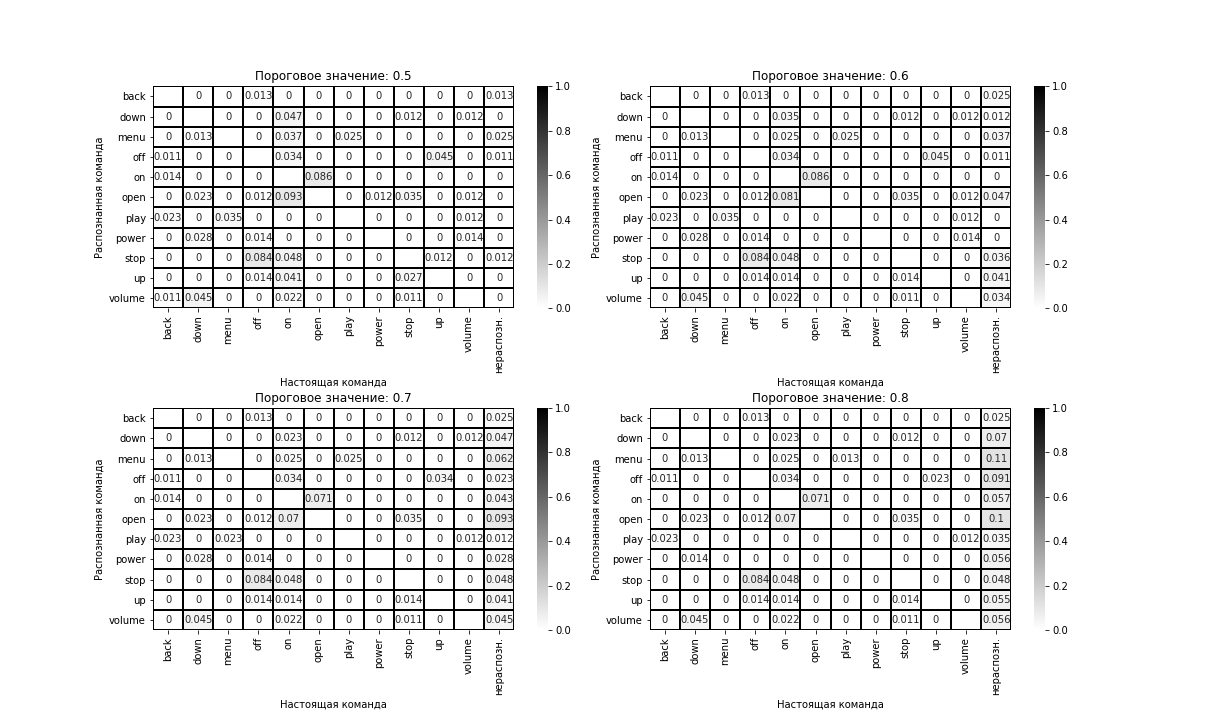
\includegraphics[scale=0.4]{cnn_cm_all_speakers.png}\]
  \caption{Матрицы ошибок для случая обучения на all\_speakers}
  \label{fig:cnn_cm_all_speakers}
\end{figure}

Видно, что при обучении только на одном дикторе, распознавание на всех остальных работает плохо. 

При обучении только на мужских голосах, распознавание на женском работает лучше, чем при обучении на одном, но все-равно очень плохо.

При обучении на всех голосах, распознавание на каждом голосе дает приемлемую точность. Однако стоит отметить, что если большая часть голосов в тренировочной части - мужские, то на женском голосе распознавание будет работать хуже, чем на мужских.